\documentclass{beamer}
%
% Choose how your presentation looks.
%
% For more themes, color themes and font themes, see:
% http://deic.uab.es/~iblanes/beamer_gallery/index_by_theme.html
%
\mode<presentation>
{
  \usetheme{Darmstadt}      % or try Darmstadt, Madrid, Warsaw, ...
  \usecolortheme{beaver} % or try albatross, beaver, crane, ...
  \usefonttheme{serif}  % or try serif, structurebold, ...
  \setbeamertemplate{navigation symbols}{}
  \setbeamertemplate{caption}[numbered]
} 

\usepackage[english]{babel}
\usepackage[utf8x]{inputenc}
\usepackage{xcolor}
\usepackage{listings}
\lstset
{
    language=[LaTeX]TeX,
    breaklines=true,
    basicstyle=\tt\scriptsize,
    %commentstyle=\color{green}
    keywordstyle=\color{blue},
    %stringstyle=\color{black}
    identifierstyle=\color{magenta},
}

\title[Management Interface]{API design and implementation of a management interface for SDN whitebox switches }
\author{Rubens Figueiredo}
\institute{FEUP}
\date{\today}

\AtBeginSection[]
{
  \begin{frame}<beamer>
    \frametitle{Outline}
    \tableofcontents[currentsection,currentsubsection]
  \end{frame}
}

\graphicspath{{../doc/figures/}}

\begin{document}

\begin{frame}
  \titlepage
        \includegraphics[width=.3\textwidth,left]{{uporto-feup}}
        \includegraphics[width=.2\textwidth,height=2cm,right]{{bisdn-logo}}
\end{frame}

% Uncomment these lines for an automatically generated outline.
\begin{frame}{Outline}
  \tableofcontents
\end{frame}

\section{Introduction}

\begin{frame}{Motivation}
    \begin{figure}
        \centering
        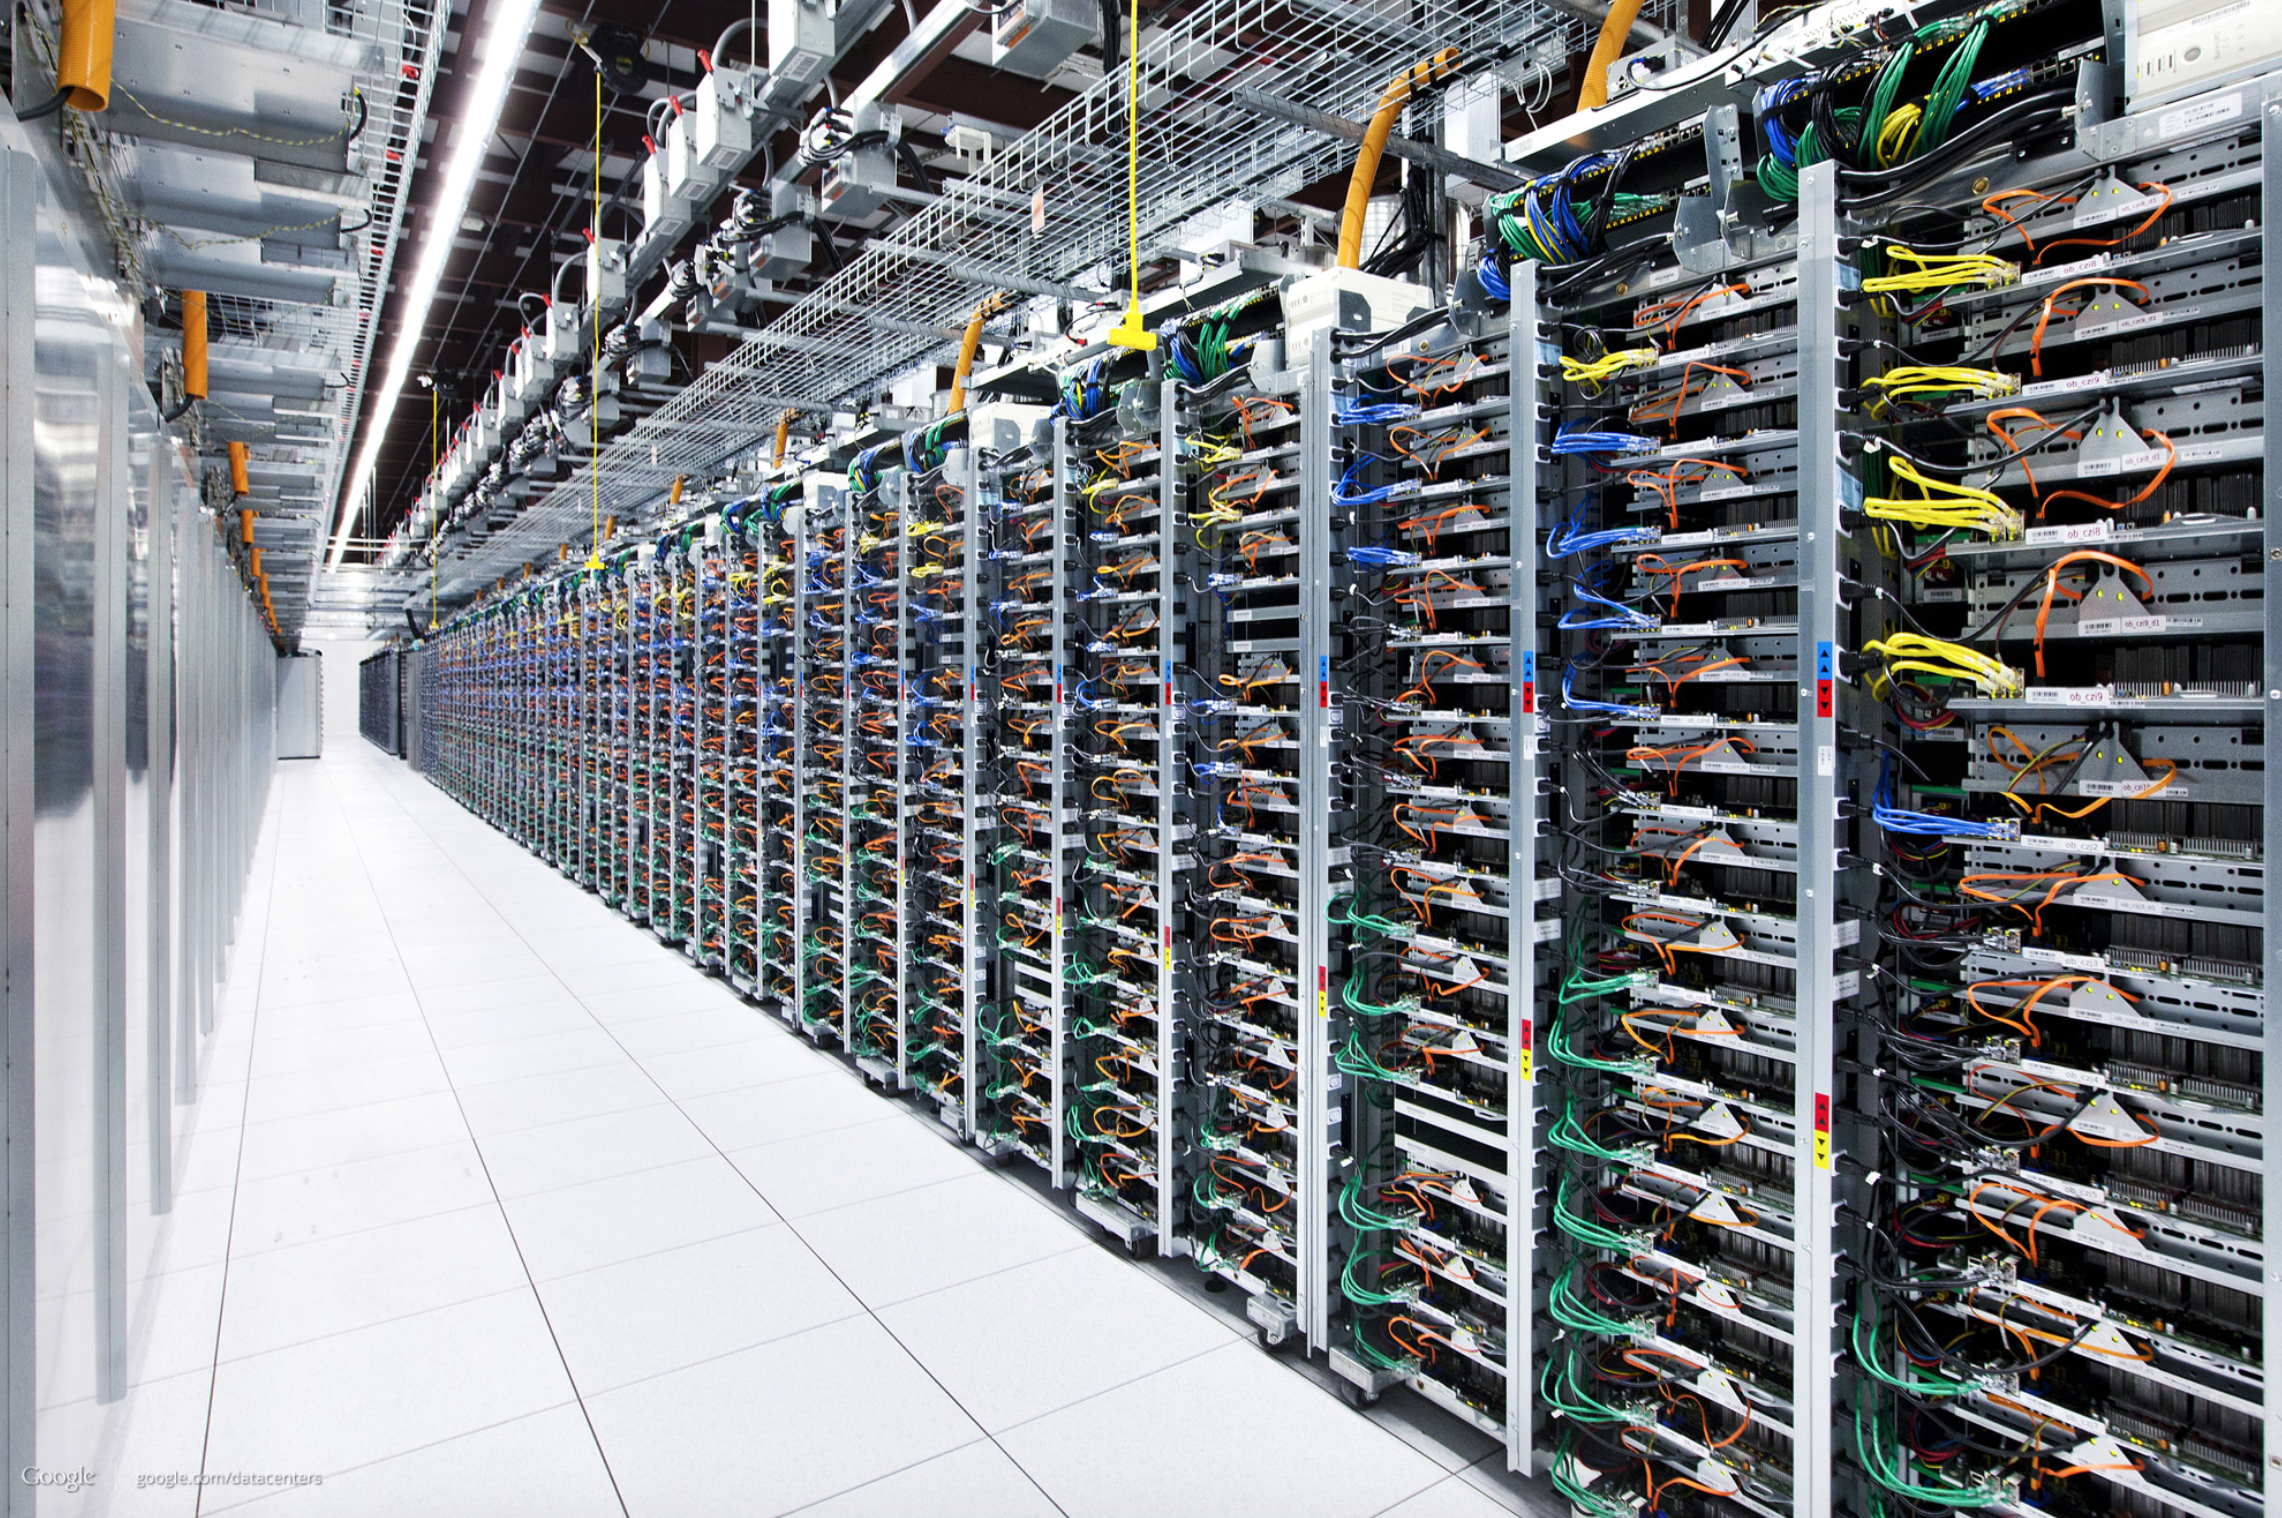
\includegraphics[width=.8\textwidth]{presentation/google_data_center}
    \end{figure}
\end{frame}

\begin{frame}{Motivation}
	\begin{itemize}
  		\item Large scale Data Center Networks are hard to operate at a highly efficient and cost effective way
        \item Individually managing each network device (switches, server, ...) is a time consuming task
  		\item Move to cloud based environments requires planning and research to create a scalable and simple environment
	\end{itemize}
\end{frame}

\begin{frame}{Software Defined Networking}
    \begin{itemize}
    \item Networking services are bound to a fast changing environment, there is a need for a network design methodology that supports this
        fast evolution
        \pause
    \item \textbf{Software Defined Networking} is a solution that provides:
        \pause
    \item \textbf{Separation of control and data planes} 
        \pause
    \item \textbf{Centralization of network management functions}
    \end{itemize}
\end{frame}

\begin{frame}
    \begin{figure}[!tbph]
      \centering
      \subfloat{\includegraphics[width=0.4\textwidth]{bib/network_trad}\label{fig:net_trad}}
      \subfloat{\includegraphics[width=.4\textwidth]{bib/network_sdn}\label{fig:net_sdn}}
      \caption {Traditional vs SDN network architecture}
    \end{figure}
\end{frame}

\begin{frame}
    \begin{figure}[!tbph]
        \centering
        \includegraphics[width=.5\textwidth]{sdn/sdn_division}
    \end{figure}
    \begin{itemize}
        \item The SDN controller plays a central role in this architecture by connecting the network applications that connect to the Northbound interface to the
            networking devices running on the Southbound plane
    \end{itemize}
\end{frame}

\begin{frame}{Basebox}
\end{frame}

\begin{frame}{Basebox}
    \begin{figure}[!tbph]
        \centering
        \includegraphics[width=.35\textwidth]{bisdn/baseboxd}
    \end{figure}

\end{frame}

\begin{frame}{Basebox}
    \begin{figure}[!tbph]
        \centering
        \includegraphics[width=.7\textwidth]{bisdn/cawr}
    \end{figure}

\end{frame}
\section{Problem}
\section{Elphant Flow Monitoring}
\section{Management API}
\end{document}
